\subsection{Cube complexes}
\label{sec:complex}

We are now able to define the central object of our thesis: CAT(0) cube complexes. First, we will introduce Euclidean cubes and some necessary notation (faces and links). Afterwards, we will define the gluing process that will lead to cube complexes. We will state some basic properties and define flag complexes. This allows us to connect the geometric property of being CAT(0) to a purely combinatorial notion which is stated in Gromov's link condition. Lastly, we will turn towards locally countable complexes and prove some necessary lemmas concerning the countability of vertex sets.

\begin{defin}[Cubes]
  A subset \(C = [0,1]^n \subset \E^n\) is called a \emph{cube}. A \emph{face} is a subset of the form 
  \[
    F = C \cap \{x_{i_1} = e_1, \dots x_{i_k} = e_k\},
  \]
  where \(k\geq0\), \(i_1, \dots, i_k\) are pairwise different elements of \(\{1, \dots, n\}\) and \(e_j \in \{0, 1\}\). \(\F\) is called a \emph{proper face} if \(F \neq C\). The notation \(F \preceq C\) will be applied for faces. The \emph{dimension} of \(F\) is \(n - k\). The \emph{interior} \(\mathring F\), is the interior of \(F\) equipped with its \(\E^{n-k}\)-structure. Any subset \(C \cap \{x_i = \text{\nfrac 1/2}\}\) is called a \emph{midcube of \(C\)}. The \emph{\(m\)-skeleton of \(C\)} is defined by
  \begin{align*}
    C^{(m)} \coloneqq \bigcup \{F \mid F \preceq C \text{ and } \dim F \leq m\}.
  \end{align*}

  Fix \(x \in C\). The \emph{support of \(x\)}, \(\supp(x)\), is the unique face of \(C\) containing \(x\) in its interior or alternatively the unique face with minimal dimension containing \(x\).

  The \emph{link of \(x\) in \(C\)} is given by
  \begin{align*}
    \lk(x,C) \coloneqq \{u \in U_x\E^n \mid \exists t > 0 \colon \exp_x(tu) \in C\} \subset U_x\E^n \cong \sphere^{n-1},
  \end{align*}
  where \(U_x\E^n\) is the unit tangent space at \(x\) in \(\E^n\) considered as a Riemannian manifold. It can be isometrically identified with \(\sphere^{n-1}\).
\end{defin}

\begin{rem}
  \(\lk(v,C) \subset \sphere^{n-1}\) is a simplex for all vertices \(v \in C\). In this case all its edges have length \(\frac{\pi}{2}\).
\end{rem}

Now, that we have introduced the vocabulary concerning Euclidean cubes, we turn towards cube complexes. These are obtained by gluing \emph{disjoint} cubes along their faces via \emph{isometries}. These restrictions ascertain that many of the combinatorial properties we know from simplicial complexes will transfere to cube complexes.

\begin{defin}[Cube complexes]\ 
  \begin{itemize}
  \item Let \((C_\lambda)_{\lambda \in \Lambda}\) be a family of cubes and \(\mathcal{C} \coloneqq \bigsqcup_{\lambda \in \Lambda} C_\lambda\) its disjoint union. Furthermore, let \(\sim\) denote an equivalence relation on \(\mathcal{C}\) and by \(X\) the space of equivalence classes with natural projection \(p \colon \mathcal{C} \to X\). Lastly, let \(p_\lambda \colon C_\lambda \to X\) be the embedding of \(C_\lambda\) into \(\mathcal{C}\) concatenated with the projection.

    \(X\) is called a \emph{cube complex}, if
    \begin{enumerate}
    \item \(p_\lambda\) is injective and
    \item for arbitrary \(\lambda_1, \lambda_2 \in \Lambda\) and \(x_i \in C_{\lambda_i}\) such that \(p_{\lambda_1}(x_1) = p_{\lambda_2}(x_2)\), there exists an isometry \(h\colon \supp(x_1) \to \supp(x_2)\), such that \(p_{\lambda_1}|_{\supp(x_1)} = p_{\lambda_2} \circ h\).
    \end{enumerate}
  \item \(C \subset X\) is called an \emph{\(n\)-dimensional cube}, if it is the image of an \(n\)-dimensional face \(F \preceq C_\lambda\) under \(p_\lambda\). The interior of \(C\) is given by \(\mathring C \coloneqq p_\lambda(\mathring F)\). A \emph{midcube of \(C\)} is the image under \(p_\lambda\) of a midcube of \(F\).
  \item The \emph{m-skeleton} of \(X\) is given by
    \begin{align*}
      X^{(m)} \coloneqq \quot{\bigsqcup_{\lambda \in \Lambda} C_\lambda^{(m)}}{\sim},
    \end{align*}
    where \(\sim\) is given by the restriction of the equivalence relation on \(\mathcal{C}\) to the disjoint union of the \(m\)-skeleta of the cells.

  % \item Fix \(x \in X\). Then the \emph{star of \(x\)} is defined by
  %   \begin{align*}
  %     \st(x) \coloneqq \bigcup \left\{\mathring C \relmid C \subset X \text{ a cube and } x \in C\right\}.
  %   \end{align*}
  \item Let \((x_i)_{i \in I}\) be the family of all the points \(x_i \in C_{\lambda(i)}\) such that \(p_{\lambda(i)}(x_i) = x\). Consider the disjoint union \(\bigsqcup_{i \in I} \lk(x_i, C_{\lambda(i)}\). We define an equivalence relation: \(u_i \sim u_j\) if and only if there exist \(t_i, t_j > 0\) such that \(\exp_{x_i}(t_i u_i) \in C_{\lambda(i)}\), \(\exp_{x_j}(t_j u_j) \in C_{\lambda(j)}\) and \(p_{\lambda(i)}(\exp_{x_i}(t_i u_i)) = p_{\lambda(j)}(\exp_{x_j}(t_j u_j))\). Then the \emph{link of \(x\) in \(X\)} is given by
    \begin{align*}
      \lk(x, X) \coloneqq \quot{\bigsqcup_{i \in I} \lk(x_{\lambda(i)}, C_{\lambda(i)})}{\sim}.
    \end{align*}
  \end{itemize}
\end{defin}

\begin{rem}
  \label{rem:complex}
  \begin{itemize}
  \item In the language of \(M_\kappa\)-polyhedral complexes the link \(\lk(x, X)\) is a \(M_1\)-polyhedral complex whenever \(x\) is a vertex of \(X\). For more details see \textcite[Section~I.7]{MR1744486}. Although all the cells of \(\lk(x,X)\) consist of simplices, it might happen that \(\lk(x,X)\) is not a simplicial complex. An example is given below in Example~\ref{bsp:ccc}. 
  \item Since the cubes are glued isometrically, one can think of \(\lk(x,X)\) as being inscribed in \(X\). The key observation is that one can fix \(t_i\) respectively \(t_j\) to any (common) value smaller than 1 (one common choice is {\nfrac 1/3}). Then the maps \(p_{\lambda(i)}(\exp_{x_i}(t_i \cdot))\) induce the embedding. Vertices correspond to the intersection of the 1-skeleton with the image of this embedding and edges must lie in the 2-skeleton. For an example see Figure~\ref{fig:link}.
    \begin{figure}[htbp]
      \centering
      \begin{tikzpicture}
    [
  vertex/.style={
    circle,
    fill=blue,
    minimum size=1mm,
    inner sep=0pt
  },
  ->-/.style={
    decoration={
      markings,
      mark=at position 0.5 with {\arrow{#1}}
    },
    postaction={decorate}
  }
  ]
  \coordinate (0) at (0,0);
  \coordinate (1) at (1,0);
  \coordinate (2) at (1,1);
  \coordinate (3) at (0,1);
  \coordinate (4) at (160:1);
  \coordinate (5) at (210:1);
  \draw (0) -- (1) -- (2) -- (3) -- (0);
  \draw (0) -- (4);
  \draw (0) -- (5);
  \node (a) at (0.33,0) [vertex] {};
  \node (b) at (0,0.33) [vertex] {};
  \node (c) at (160:0.33) [vertex] {};
  \node (d) at (210:0.33) [vertex] {};
  \draw [blue] (0.33,0) arc (0:90:0.33);
  \draw [blue, dashed] (0,0.33) arc (90:360:0.33);

  \begin{scope}[shift={(4,.5)}, scale=.5]
    \node (a) at (1,0) [vertex] {};
    \node (b) at (0,1) [vertex] {};
    \node (c) at (160:1) [vertex] {};
    \node (d) at (210:1) [vertex] {};
    \draw [blue] (a) -- (b);
  \end{scope}
\end{tikzpicture}

%%% Local Variables:
%%% mode: latex
%%% TeX-master: "../Master"
%%% End:

      \caption{The left-hand side depicts a CAT(0) cube complex (black). One vertex link is inscribed into the complex via the intersection of a small sphere (blue). The right-hand side depicts the vertex link without the CAT(0) cube complex.}
      \label{fig:link}
    \end{figure}
  \item Our definition of a cube complex is not standard. Normally, the above defined object is called a cubical complex (c.\,f.~\cite[Def.~I.7.37]{MR1744486}). The difference between the two concepts lies solely in the fact, that in the cubical case we need the maps \(p_\lambda\) to be injective on the whole cube, whereas in the cube case they are only assumed to be injective on the \emph{interior} of each cube. However, as \textcite[Thm.~C.4]{MR3029427} has shown in the case of CAT(0) cube complexes the two definitions are equivalent, hence we will adopt it from the start.
  \item By definition two cubes either intersect in a common face or have an empty intersection. In this sense, they are completely analogous to simplicial complexes (c.\,f.\ Definition~\ref{defin:flag}). 
  \end{itemize}
\end{rem}

% \todo{write something about topology}

% \begin{defin}
%   \(K\) is called a \emph{cube complex}, if it is a \(M_0\)-polyhedral complex, where every cell \(C\) is given by a unit cube of arbitrary dimension.
% \end{defin}

% From now on, if not otherwise specified, all cells \(C\) will be taken to be cubes.

% \begin{lemma}
%   \label{lemma:cube-dist}
%   Let \(x \leq C\) a cell and \(\dim C > 0\). Then
%   \begin{align*}
%     d(x, C - \st(x)) =
%     \begin{cases}
%       1 & \text{if } \dim \supp(x) = 0\\
%       d(x, \partial \supp(x)) & \text{else}
%     \end{cases}
%                          .
%   \end{align*}
% \end{lemma}

% \begin{proof}
%   If \(l = 0\) then \(x\) is a vertex of \(C^k\) and any other vertex (which exist, as \(k > 0\)) has distance at least \(1\) and is by definition not contained in the star of \(x\). Hence, \(d(x, C^k - \st(x)) \leq 1\).
  
%   After a rotation of the cube, we may assume that \(x\) is the origin and hence any face \(F\) of \(C^k\), not containing \(x\) must have at least one \(\delta_i = 1\). Let \(n_F\) denote the sum of all \(\delta_i\) defining \(F\). Then for all \(y \in F\), we have
%   \begin{align*}
%     d(x,y) = |y| \geq n_F \geq 1
%   \end{align*}
%   if \(x\) is not contained in \(F\). \(C^k - \st(x)\) is compact, therefore there there exists a \(y \in C^k - \st(x)\), such that
%   \begin{align*}
%     d(x, C^k - \st(x)) = d(x, y) 
%   \end{align*}
%   holds. Furthermore, there must exist a face \(F\) containing \(y\) in its interior. By definition of \(y\), \(F\) cannot contain \(x\). Together with the above argument we yield \(d(x, C^k - \st(x)) \geq 1\), which proves the first assertion.

%   Now, let \(l\) be different from \(0\). After a rotation, we can identify \(F\) with \(C^l\). \(\partial C^l \subset C^k - \st(x)\) holds and thus we have
%   \begin{align}
%     \label{eq:dist-border}
%     d(p, C^k - \st(x) \leq d(x, \partial C^k) < 1 .
%   \end{align}
%   As above, we find a \(y \in C^k - \st(x)\), realizing the distance. \(y\) lies in the interior of some face \(G\) and, by definition, \(G\) does not have \(C^l\) as a face. First, let us assume that \(G \cup \partial C^l \neq \varnothing\). In that case there is a unique projection \(\hat y \in G \cup \partial C^l\) of \(y\) and an element \(y_\perp\) orthogonal to \(C^l\), such that \(y = \hat y + y_\perp\). Then we have
%   \begin{align*}
%     d^2(x, y) = |x - \hat y|^2 + |y_\perp|^2 \leq d(x, \hat y).
%   \end{align*}
%   Hence \(y_\perp = 0\), which leads to \(y = \hat y \in \partial C^l\). If \(G \cup \partial C^l = \varnothing\), then at least one of the components \(l+1, \dots, k\) have to be fixed to \(1\), leading to \(d(x, C^k - \st(x)) = d(x,y) \geq 1\), which is a contradiction to Equation~\ref{eq:dist-border}, which proves the other inequality.
% \end{proof}

% \begin{lemma}
%   If \(K\) is a cube complex, then \(\epsilon(x) > 0\) (c.\,f.~\eqref{eq:epsilon}) for arbitrary \(x \in K\).
% \end{lemma}

% \begin{proof}
%   By definition of a cube complex, for any point \(x\) and two preimages \(x_i \in C_{\lambda_i}\), we have an isometry \(h \colon \supp(x_1) \to \supp(x_2)\). Hence, for any \(F_i \leq C_{\lambda_i}\), we have that \(d(x_1, F_1 \setminus \st(x_1)) = d(x_2, F_2 \setminus \st(x_2))\) by Lemma~\ref{lemma:cube-dist}. This shows that \(d(x, C \setminus \st(x))\) can be computed in any preimage of the cell \(C\) and furthermore, that the value is independent of \(C\). Hence, \(\epsilon(x) > 0 \).
% \end{proof}

In the following we will list some useful results about cube complexes. For the proofs see~\cite[Appendices A, B]{MR3029427}. For the finite dimensional case we refer to~\cite[Sec. I.7, II.5]{MR1744486}.

\begin{thm}[{\cite[I.7.10]{MR1744486}}]
  \label{thm:metric}
  Every cube complex \(X\) is a metric space, when equipped with path metric \(d\) induced by the piecewise linear paths in \(X\).
\end{thm}

% \begin{proof}
%   The symmetry in triangle enequality follow directly from the definition. It remains to prove that \(d(x,y) = 0\) implies \(x = y\). In order to do that, we claim that if \(d(x,y) < \epsilon(x)\), then there exists a cube \(C \subset K\), such that \(x, y \in C\) with preimages \(\bar x, \bar y \in C_\lambda\) such that \(d(x,y) = d_{C_\lambda}(\bar x,\bar y)\). The claim then follows directly. However, we will not show this claim directly but further reduce the assertion. We consider \(m\)-strings \(s \coloneqq (x_0, \dots, x_m) \in K^{m+1}\), with the property that each sucessive pair of points \(x_{i-1}, x_i\) are contained in a common cube \(C_i\). With this we define the length of a string as \(l(s) = \sum_{i=1}^n d_{C_i}(x_{i-1}, x_i)\), where \(d_{C_i}\) is the metric on \(C_i\) induced by any of its preimages under the natural projection.

%   These \(m\)-strings are in \(1:1\)-correspondence with piecwiese geodesic segments in \(K\) and thus we can use the two notions interchangeable. We will prove the claim: If \(l(s) < \epsilon(x_0)\), then there exists a cube \(C \subset K\) with \(x_0, x_m \in C\) and such that \(d_C(x_0, x_m) \leq l(s)\). We proceed by induction. For \(m=1\) the claim is true by definition. Assume that the claim is true for some \(m \in \N\) and let \(s = (x_0, \dots, x_{m+1})\) be an \((m+1)\)-string and \(s'\) the \(m\)-string consisting of the first \(m+1\) entries. By definition there exists a cube \(C\) such that \(x_m, x_{m+1} \in C\). Furthermore, \(d(x_0, x_m) \leq l(s') \leq l(s) < \epsilon(x_0)\). Hence, \(x_m \in \st(x_0)\). So there exists a second cube \(\tilde C\) that contains \(x_m\) in its interior. Also \(\tilde C \cap C\) is not empty and hence also a cube. Since \(x_m\) is in the interior of \(\tilde C\) we have \(\tilde C \subset C\) and hence \(x_0 \in C\). We have
%   \begin{align*}
%     d_C(x_0, x_{m+1}) \leq d_C(x_0, x_m) + d_C(x_m x_{m+1}) \stackrel{\ast}{\leq} l(s') + d_C(x_m + x_{m+1}) = l(s),
%   \end{align*}
%   which is what we wanted to show. For the inequality \(\ast\), we use the induction hypothesis together with the observation that if the inequality is true for any cube containing \(x_0\) and \(x_m\), then it is true for all cubes containing both points.

%   So we see that for all pairs \(x,y \in K\) with \(d(x,y) < \epsilon(x)\), we find a cube \(C\) containing both and \(d_C(x,y) \leq d(x,y)\). However, by construction of \(d\) this already implies equality. For \(d_C\) we already know that it is a metric on its cube. So \(d(x,y) = 0\) implies \(x = y\).
% \end{proof}


\begin{thm}[{\cite[Theorem A.6]{MR3029427}}, {\cite[Theorem I.7.50]{MR1744486}}]
  A cube complex is complete if and only if every chain of ascending cubes is finite.
\end{thm}

\begin{notation}
  Let \(S\) be a set. We will denote its \emph{power set} by
  \[
    \operatorname{Pot}(S) = \{A \subset S\}.
  \]
\end{notation}

\begin{defin}[Flag complexes and joins]
  \label{defin:flag}
  \begin{itemize}
  \item
    Let \(S\) be a set an \(P \subset \operatorname{Pot}(S)\). A pair \(K = (S, P)\) is called a \emph{simplicial complex} if \(\{s\} \in P\) for every \(s \in S\) and for every \(X \in P\) and \(Y \subset X\) with \(Y \neq \varnothing\) we have \(Y \in P\).

    A \emph{\(n\)-simplex} is an element \(X \in P\) such that \(|X| = n+1\).

    A \(0\)-simplex is called a \emph{vertex} and a \(1\)-simplex is called an \emph{edge}.
  \item
    A simplicial complex \(K = (S,P)\) is \emph{flag}, if every finite subset of \(S\) that is pairwise joined by edges spans a simplex (see\ \cite[Definition II.5.15]{MR1744486}).
  \item Let \(K_1 = (S_1, P_1)\) and \(K_2 = (S_2, P_2)\) be two simplicial complexes. Their \emph{join} \(K\) is the simplicial complex \((S,P)\) such that \(S \coloneqq S_1 \sqcup S_2\) and \(X \in P\) if and only if one of the following is true:
    \begin{enumerate}
    \item \(X \in P_1\),
    \item \(X \in P_2\) or
    \item there exist \(X_i \in P_i\) such that \(X = X_1 \sqcup X_2\).
    \end{enumerate}
  \end{itemize}
  We write \(K = K_1 \ast K_2\) (See\ \cite[Definition~I.7A.2]{MR1744486}).
\end{defin}

\begin{thm}[Gromov's link condition, {\cite[Theorem B.8]{MR3029427}}, {\cite[Theorem II.5.20]{MR1744486}}]
  \label{thm:link}
  A cube complex \(X\) is \emph{non-positively curved} if and only if \(\lk(v,X)\) is a flag complex for each vertex \(v \in X\).

  A cube complex \(X\) is \emph{CAT(0)} if and only if \(\lk(v,X)\)  is a flag complex for each vertex \(v \in X\) and \(X\) is simply connected.
\end{thm}

\begin{bsp}[{\cite{sageev-lecture-notes}}]
  \label{bsp:ccc}
  \begin{description}
  \item[Graphs:] The link of every vertex in a graph is a set of disconnected vertices, which is by the non-existence of any higher dimensional simplices a flag complex. Hence, every graph is non-positively curved. In the case of graphs simply connectedness is equivalent to the graph being a tree, such that we see that CAT(0) cube complexes are in a natural way a generalization of trees.
  \item[Sphere:] Figure~\ref{fig:sphere} contains three representations of the two-dimensional sphere as a quotient of a disjoint union of cubes. None of these is a CAT(0) cube complex. In case~\ref{fig:sphere-a} the cube is not embedded  into the quotient. Nonetheless, one can define a links for the vertices and we see that the these are not simplicial complexes, since one contains a loop and the other contains parallel edges. In the case~\ref{fig:sphere-b}, we see that we can indeed realize the sphere as a cube complex in our sense, however, we still have an non-simplicial vertex link. In the case~\ref{fig:sphere-c}, we can even find a realization as a cube complex such that the vertex links are simplicial. However, even then the link is not flag.

    Naturally, this is as it should be as we know that a sphere is an example of a positively curved space and our definition agrees with the one in the case of manifolds.
    \begin{figure}[htbp]
      \centering
      \subcaptionbox{\label{fig:sphere-a}}[.4\linewidth]{\begin{tikzpicture}
  [
  vertex/.style={
    circle,
    fill=black,
    minimum size=1mm,
    inner sep=0pt
  },
  ->-/.style={
    decoration={
      markings,
      mark=at position 0.5 with {\arrow{#1}}
    },
    postaction={decorate}
  }
  ]
  \node at (0,0) [vertex] {}
  edge [->-={>}] (1,0)
  node at (1,0) [vertex] {}
  edge [->-={<}] (1,1)
  node at (1,1) [vertex] {}
  edge [->-={<<}] (0,1)
  node at (0,1) [vertex] {}
  edge [->-={>>}] (0,0);
  \node at (2.5,0) [vertex] {};
  \draw (2.5,0) to [out=45,in=135,loop] (2.5,0);
  \node at (2,1) [vertex] {}
  edge [bend right] (3,1)
  node at (3,1) [vertex] {}
  edge [bend right] (2,1);
\end{tikzpicture}

%%% Local Variables:
%%% mode: latex
%%% TeX-master: "../Master"
%%% End:
}%
      \subcaptionbox{\label{fig:sphere-b}}[.4\linewidth]{\begin{tikzpicture}
  [
  vertex/.style={
    circle,
    fill=black,
    minimum size=1mm,
    inner sep=0pt
  },
  ->-/.style={
    decoration={
      markings,
      mark=at position 0.5 with {\arrow{#1}}
    },
    postaction={decorate}
  }
  ]
  \node at (0,0) [vertex] {}
  edge [->-={>}] (1,0)
  node at (1,0) [vertex] {}
  edge [->-={<}] (2,0)
  node at (2,0) [vertex] {}
  edge [->-={<<}] (2,1)
  node at (2,1) [vertex] {}
  edge [>={Stealth},->-={>}] (1,1)
  node at (1,1) [vertex] {}
  edge [>={Stealth},->-={<}] (0,1)
  node at (0,1) [vertex] {}
  edge [->-={>>}] (0,0);
  \draw (1,0) -- (1,1);
  \begin{scope}[shift={(3,0.5)}]
    \node at (0,0) [vertex] {}
    edge [bend left] (1,0)
    node  at (1,0) [vertex] {}
    edge [bend left] (0,0);
  \end{scope}
\end{tikzpicture}

%%% Local Variables:
%%% mode: latex
%%% TeX-master: "../Master"
%%% End:
}
      \subcaptionbox{\label{fig:sphere-c}}[1\linewidth]{% Sphere
\begin{tikzpicture}
  [
  vertex/.style={
    circle,
    fill=black,
    minimum size=1mm,
    inner sep=0pt
  },
  ->-/.style={
    decoration={
      markings,
      mark=at position 0.5 with {\arrow{#1}}
    },
    postaction={decorate}
  }
  ]
  \node ( 1) at ( 0, 0) [vertex] {};
  \node ( 2) at ( 0, 1) [vertex] {};
  \node ( 3) at ( 1, 0) [vertex] {};
  \node ( 4) at ( 1, 1) [vertex] {};
  \node ( 5) at ( 0, 2) [vertex] {};
  \node ( 6) at ( 1, 2) [vertex] {};
  \node ( 7) at ( 0, 3) [vertex] {};
  \node ( 8) at ( 1, 3) [vertex] {};
  \node ( 9) at (-1, 1) [vertex] {};
  \node (10) at (-1, 2) [vertex] {};
  \node (11) at ( 2, 1) [vertex] {};
  \node (12) at ( 2, 2) [vertex] {};
  \node (13) at ( 3, 1) [vertex] {};
  \node (14) at ( 3, 2) [vertex] {};
  \draw[->-=>] (0,0) -- (1,0);
  \draw[->-=>>] (1,0) -- (1,1);
  \draw[->-=<<] (1,1) -- (2,1);
  \draw[->-=<] (2,1) -- (3,1);
  \draw[>={Stealth}, ->-=>] (3,1) -- (3,2);
  \draw[>={Stealth}, ->-=<<] (3,2) -- (2,2);
  \draw[>={triangle 45}, ->-=>] (2,2) -- (1,2);
  \draw[>={triangle 45}, ->-=<] (1,2) -- (1,3);
  \draw[>={Stealth}, ->-=>>] (1,3) -- (0,3);
  \draw[>={triangle 45}, ->-=<<] (0,3) -- (0,2);
  \draw[>={triangle 45}, ->-=>>] (0,2) -- (-1,2);
  \draw[>={Stealth}, ->-=<] (-1,2)-- (-1,1);
  \draw[>={open triangle 45}, ->-=>] (-1,1) -- (0,1);
  \draw[>={open triangle 45}, ->-=<] (0,1) -- (0,0);
  \draw (0,1) -- (1,1) -- (1,2) -- (0,2) -- (0,1);
  \draw (2,2) -- (2,1);


  \node at (0,3.5) {\phantom{v}};
  
  \begin{scope}[shift={(4.5,1)}]
    \node at (0,0) [vertex] {}
    edge (1,0)
    node at (1,0) [vertex] {}
    edge (0.5, 0.87)
    node at (0.5, 0.87) [vertex] {}
    edge (0,0);
  \end{scope}
\end{tikzpicture}

%%% Local Variables:
%%% mode: latex
%%% TeX-master: "../Master"
%%% End:
}%
      \caption{Three topological realizations of a sphere and their vertex links. Figure~\subref{fig:sphere-a} is not a cube complex, whereas Figures~\subref{fig:sphere-b} and~\subref{fig:sphere-c} are. In Figure~\subref{fig:sphere-b} the link is not a simplicial complex (parallel edges). In Figure~\subref{fig:sphere-c} the link is simplicial, but still not flag.}
      \label{fig:sphere}
    \end{figure}
  \item[Torus:] Figure~\ref{fig:torus} contains a realization of a two-dimensional torus as a cube complex. The vertex links show that the torus is indeed non-positively curved. This is what we would expect, since a torus is an example of a flat space. However, it is not a CAT(0) cube complex, as it is not simply connected. A generalization of the Cartan-Hadamard theorem shows that the universal cover of a non-positively curved cube complex is always CAT(0). In the case of a torus the universal cover can be chosen to be \(\R^2\) with its standard cubulation via \(\Z^2\).
    \begin{figure}[htbp]
      \centering
      % Torus
\begin{tikzpicture}
  [vertex/.style={circle,fill=black, minimum size=1mm, inner sep=0pt}]
  \draw [>-   ] (-2, 2) -- (-1, 2) (-1, 2) -- ( 0, 2);
  \draw [>-   ] (-2,-2) -- (-1,-2) (-1,-2) -- ( 0,-2);
  \draw [>>-  ] ( 0, 2) -- ( 1, 2) ( 1, 2) -- ( 2, 2);
  \draw [>>-  ] ( 0,-2) -- ( 1,-2) ( 1,-2) -- ( 2,-2);
  \draw [>={Stealth},>- ] ( 2,-2) -- ( 2,-1) ( 2,-1) -- ( 2, 0);
  \draw [>={Stealth},>- ] (-2,-2) -- (-2,-1) (-2,-1) -- (-2, 0);
  \draw [>={Stealth},>>-] ( 2, 0) -- ( 2, 1) ( 2, 1) -- ( 2, 2);
  \draw [>={Stealth},>>-] (-2, 0) -- (-2, 1) (-2, 1) -- (-2, 2);
  \draw [dashed] ( 0, 2) -- ( 0,-2);
  \draw [dashed] ( 2, 0) -- (-2, 0);
  \node at ( 0, 0) [vertex,draw,label= 45:\(x\)] {};
  \node at ( 2, 0) [vertex,draw,label=135:\(z_1\)] {};
  \node at (-2, 0) [vertex,draw,label= 45:\(z_1\)] {};
  \node at ( 0, 2) [vertex,draw,label=315:\(z_2\)] {};
  \node at ( 0,-2) [vertex,draw,label= 45:\(z_2\)] {};
  \node at ( 2, 2) [vertex,draw,label=225:\(y\)] {};
  \node at (-2,-2) [vertex,draw,label= 45:\(y\)] {};
  \node at (-2, 2) [vertex,draw,label=315:\(y\)] {};
  \node at ( 2,-2) [vertex,draw,label=135:\(y\)] {};
\end{tikzpicture}
% \hfill{}
\hspace{2cm}
% link of torus
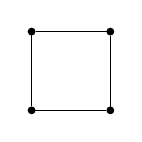
\begin{tikzpicture}
  [
  vertex/.style={
    circle,
    fill=black,
    minimum size=1mm,
    inner sep=0pt
  }
  ]
  \node at (0,0) [vertex] {}
  edge (0,1)
  node at (0,1) [vertex] {}
  edge (1,1)
  node at (1,1) [vertex]{}
  edge (1,0)
  node at (1,0) [vertex]{}
  edge (0,0);
\end{tikzpicture}



%%% Local Variables:
%%% mode: latex
%%% TeX-master: "../Master"
%%% End:

      \caption{Realization of a 2-dimensional torus as a cube complex and its vertex link. We see that the torus is non-positively curved.}
      \label{fig:torus}
    \end{figure}

    The above considerations generalize to tori in arbitrary dimensions.
  \item[Higher genus surfaces:] In order to complete our discussion of surfaces, we consider in Figure~\ref{fig:genus-2} the example of a genus 2 surface. Inscribed in the standard octagon, there are four more geodesics creating eight cubes embedded in the quotient. The vertex links are clearly flag and so we see that the surface can be realized as a non-positively curved cube complex. The construction can be generalized to all higher genus surfaces. This is expected, as all these higher genus surfaces are negatively curved.
    \begin{figure}[htbp]
      \centering
      % Genus 2
\begin{tikzpicture}
  [
  vertex/.style={
    circle,
    fill=black,
    minimum size=1mm,
    inner sep=0pt
  },
  ->-/.style={
    decoration={
      markings,
      mark=at position 0.4 with {\arrow{#1}}
    },
    postaction={decorate}
  }
  ]
  \node (1) at ( 2, 0) [vertex, label=0:\(x_2\)] {};
  \node (2) at ( 1.41, 1.41) [vertex, label=45:\(x_2\)] {}
  edge [bend right, ->-=>] (1);
  \node (3) at ( 0, 2) [vertex, label=90:\(x_2\)] {}
  edge [bend right, ->-=>>] (2);
  \node (4) at (-1.41, 1.41) [vertex, label=135:\(x_2\)] {}
  edge [bend right, ->-=<] (3);
  \node (5) at (-2, 0) [vertex, label=180:\(x_2\)] {}
  edge [bend right, ->-=<<] (4);
  \node (6) at (-1.41,-1.41) [vertex, label=225:\(x_2\)] {}
  edge [bend right, ->-={Stealth}] (5);
  \node (7) at ( 0,-2) [vertex, label=270:\(x_2\)] {}
  edge [bend right, >=Stealth, ->-={>>}] (6);
  \node (8) at ( 1.41,-1.41) [vertex, label=135:\(x_2\)] {}
  edge [bend right, >=Stealth, ->-={<}] (7)
  edge [bend left,>=Stealth, ->-={>>} ] (1);
  \node at (22.5:1.6) [vertex, label=22.5:\(z_1\)] {}
  edge [dashed] (202.5:1.6)
  node at (202.5:1.6) [vertex, label=202.5:\(z_3\)] {};
  \node at (67.5:1.6) [vertex, label=67.5:\(z_2\)] {}
  edge [dashed] (247.5:1.6)
  node at (247.5:1.6) [vertex, label=247.5:\(z_4\)] {};
  \node at (112.5:1.6) [vertex, label=112.5:\(z_1\)] {}
  edge [dashed] (292.5:1.6)
  node at (292.5:1.6) [vertex, label=292.5:\(z_3\)] {};
  \node at (157.5:1.6) [vertex, label=157.5:\(z_2\)] {}
  edge [dashed] (337.5:1.6)
  node at (337.5:1.6) [vertex, label=337.5:\(z_4\)] {};
  \node at ( 0, 0) [vertex,label=45:\(x_1\)] {};

  \begin{scope}[shift={(4,-1.5)}]
    \node at (0.5, -1) {\(\lk(x_i)\)};
    \node at (0,0) [vertex] {}
    edge (1,0)
    node at (1,0) [vertex] {}
    edge (1,1)
    node at (1,1) [vertex] {}
    edge (1,2)
    node at (1,2) [vertex] {}
    edge (1,3)
    node at (1,3) [vertex] {}
    edge (0,3)
    node at (0,3) [vertex] {}
    edge (0,2)
    node at (0,2) [vertex] {}
    edge (0,1)
    node at (0,1) [vertex] {}
    edge (0,0);
    \begin{scope}[shift={(1,0)}]
      \node at (2.5,-1) {\(\lk(z_i)\)};
      \node at (2,0) [vertex] {}
      edge (3,0)
      node at (3,0) [vertex] {}
      edge (3,1)
      node at (3,1) [vertex] {}
      edge (2,1)
      node at (2,1) [vertex] {}
      edge (2,0);
    \end{scope}
  \end{scope}
\end{tikzpicture}

%%% Local Variables:
%%% mode: latex
%%% TeX-master: "../Master"
%%% End:

      \caption{Realization of a genus 2 surfaces as a cube complex and the two non-isomorphic vertex links. As can be seen the surface is non-positively curved.}
      \label{fig:genus-2}
    \end{figure}

    As in the previous example, these surfaces lead to a cube complex structure on the universal cover, which can be chosen to be \(\mathbb{H}^2\).
  \end{description}
\end{bsp}

\begin{lemma}
  \label{lem:flag}
  The join \(K = (S,P)\) of two simplicial complexes \(K_1 = (S_1, P_1)\) and \(K_2 = (S_2, P_2)\) is a simplicial complex. If \(K_1\) and \(K_2\) are flag, so is \(K\).
\end{lemma}

\begin{proof}
  Let \(X \in P\) and \(\varnothing \neq Y \subset X\). The set \(X\) can be decomposed as \(X = X_1 \sqcup X_2\), where \(X_i \in P_i\). With this we have \(Y = Y_1 \sqcup Y_2\) where \(Y_i \coloneqq X_i \cap Y\). Since \(Y\) is non-empty not both \(Y_i\) can be empty. If both are non-empty then we have \(Y_i \in P_i\) and thus \(Y \in P\) (We use that the \(K_i\) are simplicial complexes). If one is empty (without loss of generality assume \(Y_2 = \varnothing\)), then \(Y = Y_1 \in P_1 \subset P\). We conclude that \(K\) is a simplicial complex.

  We will now show that \(K\) is flag. Let \(v_1, \dots, v_n \in P\) be distinct vertices that are pairwise connected in the 1-skeleton, i.\,e.\ \(v_i \cup v_j \in P\) for all \(i \neq j\). We have to show that \(X \coloneqq \bigcup_i v_i \in P\). After renaming the vertices we may assume that \(v_1, \dots, v_k \in P_1\) and \(v_{k+1}, \dots v_{n} \in P_2\). If \(k=0\) or \(k=n\), we are done as the \(K_i\) is flag and we have \(P_i \subset P\). Otherwise \(X_1 \coloneqq \bigcup_{i=1}^kv_i \in P_1\) and \(X_2 \coloneqq \bigcup_{i=k+1}^n v_i \in P_2\), again since the \(K_i\) are flag. However, then \(X = X_1 \cup X_2 \in P\) by definition. Hence \(K\) is flag.
\end{proof}

\begin{prop}
  \label{prop:product-cat}
  Let \(X_1\) and \(X_2\) be two cube complexes then \(X \coloneqq X_1 \times X_2\) is a cube complex. If \(X_1\) and \(X_2\) are both CAT(0), so is \(X\).
\end{prop}

\begin{proof}
  We will first prove that \(X_1 \times X_2\) is a cube complex. If \(X_1\) and \(X_2\) are cube complexes, we have the following maps:
  \begin{align*}
    p_i \colon \bigsqcup_{\lambda \in \Lambda_i} C_\lambda \to X_i
  \end{align*}
  Hence, we have the map
  \[
    (p_1 \times p_2) \colon \bigsqcup_{\lambda' \in \Lambda_1} \bigsqcup_{\lambda \in \Lambda_2} C_{\lambda'} \times C_{\lambda} \to X_1 \times X_2
  \]
  and via the embedding of the cubes the maps
  \[
    p_{\lambda', \lambda} \colon C_{\lambda'} \times C_{\lambda} \to X_1 \times X_2.
  \]
  These maps are injective because each \(p_i\) is on every cube. We will now prove that the glue by isometries. However, this also works on each factor separately.

  We turn towards the prove that \(X\) is CAT(0). We will show that for any vertex \((v,w) \in X\) the link \(\lk((v,w), X)\) is the join of \(\lk(v, X_1)\) and \(\lk(w,X_2)\). We use Remark~\ref{rem:complex} and think of the link as inscribed into the complex. Let us start with two Euclidean cubes \(C_{\lambda'}\) and \(C_\lambda\) and the origin as the vertex. Let \(n = \dim C_{\lambda'}\) and \(k = \dim C_\lambda\). Then a vertex \(v \in \lk(0, C_{\lambda'} \times C_{\lambda})\) is uniquely defined by the unique coordinate \(v_i\) which is non-zero. If \(i \leq n\) then \(v\) corresponds to a vertex in \(\lk(0, C_{\lambda'})\), otherwise to a vertex in \(\lk(0, C_\lambda)\). Now, the three links are indeed a \((n-1)\)-, \((k-1)\)- and \((n+k-1)\)-simplex and we have \(\lk(0, C_{\lambda'} \times C_\lambda) = \lk(0, C_{\lambda'}) \ast \lk(0, C_{\lambda})\).

  In the case of a general \(X\), we can accomplish the above decomposition on each cube separately. Since the isometric gluing is also factor wise, it preserves the decomposition and we have \(\lk((v,w), X) = \lk(v, X_1) \ast \lk(v, X_2)\). With this assertion in place Lemma~\ref{lem:flag} finishes the proof.
\end{proof}

The above proposition leads to the following definition:

\begin{defin}
  A CAT(0) cube complex \(X\) is called \emph{reducible}, if it can be decomposed as a (proper) product of CAT(0) cube complexes. Otherwise, it is called \emph{irreducible}.
\end{defin}

\begin{defin}
  A cube complex \(X\) is called \emph{locally finite} if every \(x \in X\) is contained in only finitely many cubes. It is called \emph{locally compact} if for every \(x \in X\) there exists a compact neighborhood \(K \subset X\). It is called \emph{locally countable} if every \(x \in X\) is contained in at most countably many cubes.
\end{defin}

\begin{prop}[{\cite[Prop.~14]{Rolli2012}}]
  Let \(X\) be a cube complex. Then the following are equivalent:
  \begin{enumerate}
  \item \(X\) is locally finite,
  \item each bounded subset of \(X\) meets only finitely many cubes,
  \item \(X\) is proper (i.\,e.\ closed balls are compact) and
  \item \(X\) is locally compact.
  \end{enumerate}
\end{prop}

\begin{lemma}
  \label{lem:lf-countable}
  If \(X\) is a locally countable CAT(0) cube complex. Let \(V(X)\) be its vertex set equipped with the edge metric \(d\). Then for every \(x_0 \in V(X)\) and \(n \in \N_0\) the set \(X_n \coloneqq \{x \in V(X) \mid d(x_0, x) = n\}\) is countable.
\end{lemma}

\begin{proof}
  We fix \(x_0 \in V(X)\) and proceed by induction. Since \(d\) is a metric we have \(X_0 = \{x_0\}\). Now, assume \(X_n\) to be countable and let for each \(x \in V(X)\) be \(N(x)\) the set of its neighboring vertices (i.\,e.\ all vertices connected by an edge to \(x\) or equivalently all vertices with distance 1 from \(x\)). Because of the local countability \(N(x)\) is countable. Thus
  \[
    X_{n+1} \subset \bigcup_{x \in X_n} N(x)
  \]
  is a countable set.
\end{proof}

\begin{rem}
  In this thesis we will be mostly concerned with connected, locally countable, finite-dimensional CAT(0) cube complexes. We will recall in each section which assumptions are necessary on our space.
\end{rem}

\subsection{Combinatorial maps}
\label{sec:comb-map}

This is a very short section concerned with maps between cube complexes. We will deal with these maps in order to understand group actions on CAT(0) cube complexes and the decomposition of the complexes in factors.

\begin{defin}[Combinatorial maps]
  \label{def:morphism-ccc}
  Let \(X,Y\) be cube complexes. The map \(f\colon X \to Y\) is called a \emph{morphism of cube complexes} or a \emph{combinatorial map}, if
  \begin{enumerate}
  \item each vertex \(v \in X^{(0)}\) is mapped to a vertex \(f(v) \in Y^{(0)}\),
  \item each cube \(C \subset X\) is mapped to a cube \(f(C) \subset Y\) and
  \item the induced map given by
    \[
      f_{\lambda, \omega}\colon C_\lambda \xrightarrow{p_{X,\lambda}} C \xrightarrow{f} f(C) \xrightarrow{p^{-1}_{Y,\omega}} C_\omega
    \]
    can be represented as \(f_{\lambda,\omega}(x) = \sum_{i=1}^n a_i f(v_i)\), where \(v_1, \dots, v_n\) are the vertices of \(C_\lambda\) and \(x = \sum_{i=1}^n a_i v_i\) is an arbitrary element of \(C_\lambda\) in its convex representation.
  \end{enumerate}
  The automorphism group of a cube complex \(X\) will be denoted by \(\Aut(X)\).
\end{defin}

\begin{rem}
  The above definition of a combinatorial map is completely analogous to the one of a simplicial map of simplicial complexes (confer for example~\cite{Singer}).
\end{rem}

\begin{lemma}
  After possibly rotating \(C_\lambda \subset \R^n\) and \(C_\omega \subset \R^m\), the map \(f_{\lambda, \omega}\) is induced by the restriction of the natural projection from \(\R^n\) to \(\R^m\). In particular we have \(n \geq m\).
\end{lemma}

\begin{cor}
  The map \(f_C\colon C \to Y\) is distance non-increasing for each cube \(C \subset X\).
\end{cor}

\begin{prop}
  Let \(f\colon X \to Y\) be a combinatorial map. Then \(f\) is distance non-increasing, i.\,e.\ \(d_Y(f(x), f(y)) \leq d_X(x,y)\) for all \(x,y \in X\). In particular a combinatorial isomorphism is an isometry.
\end{prop}

\begin{proof}
  By the combinatorial structure of \(f\) each piecewise linear path \(c\) in \(X\) is mapped to a piecewise linear path in \(Y\). For each \(x,y \in X\) we denote by \(\operatorname{PL}(x,y)\) the piecewise linear paths joining \(x\) to \(y\). Furthermore, each segment of \(c\) lying in a cube is shortened by the previous corollary. Hence, \(l(f \circ c) \leq l(c)\) and thus
  \begin{align*}
    d_X(x,y)
    & = \inf\left\{l(c) \relmid c \in \operatorname{PL}(x,y)\right\}\\
    & \geq \inf\left\{l(f \circ c) \relmid c \in \operatorname{PL}(x,y)\right\}\\
    & \geq \inf\left\{l(c) \relmid c \in \operatorname{PL}(f(x), f(y))\right\}\\
    & = d_Y(x,y),
  \end{align*}
  which is the desired result.
\end{proof}

% \begin{lemma}
%   Let \(f\colon X \to Y\) be a combinatorial map and a local homeomorphism between cube complexes. Then \(f|_C\colon C \to f(C)\) is an isometry for every cube \(C \subset X\) and \(f\) is a local isometry.
% \end{lemma}

% \begin{proof}
%   For the first assertion consider \(x \in \mathring{C}\) and a open neighborhood \(U\) of \(x\) such that \(f|_U\) is a homeomorphism. Let \(v_1, \dots, v_n \in C\) be the vertices of \(C\). Then, using these coordinates, we can write \(x = \sum_i a_i v_i\) with \(a_i\) coefficients of the convex combination and \(f\) takes the form
%   \[
%     f(x) = \sum_i a_i f(v_i).
%   \]
%   Assume that \(f(v_1), \dots, f(v_n)\) are not pairwise different. That means without loss of generality we have \(f(v_1) = f(v_2)\). Let \(\epsilon > 0\) and define
%   \[
%     y \coloneqq \sum_i b_i v_i \quad \text{with } b_i = \begin{cases}a_1 + \epsilon & i = 1\\a_2 - \epsilon & i = 2\\ a_i & \text{else}\end{cases}.
%   \]
%   Since \(U\) is open and \(x \in \mathring{C}\), we can choose \(\epsilon\) small enough such that \(y \in U \cap C\), but by construction we have \(f(y) = f(x)\), which is a contradiction to the fact that \(f|_U\) is homeomorphism. Hence the \(f(v_i)\) need to be pairwise differnt, but this is already sufficient to show that \(f|_C\) is an isometry.

%   For the second claim consider \(z \in X\). Then there exists an \(\epsilon(z)\) such that each \(y \in B(z, \epsilon(z))\) and \(z\) lie in a common cube (c.\,f.~\cite[I.7.8-9]{MR1744486}) and by \textcite[I.7.33]{MR1744486} we have that it is always positve. Let \(0 < \epsilon \leq \epsilon(z)\), such that \(f\) is a homeomorphism \(B \coloneqq B(z, \epsilon)\). Set \(\tilde B \coloneqq f(B)\) and let \(\tilde x, \tilde y \in \tilde B \cap \tilde C\), where \(\tilde C\) is some cube in \(Y\). Then we find unique preimages \(x\) and \(y\) in \(B\).
%   Assume there is no common cube containing both \(x\) and \(y\).
%   Let us consider the case that \(\tilde x \in \supp(\tilde y) \subset \tilde C\) and consider \(C = \supp(y)\) and \(C' = \supp(x)\). Then \(f|_C\colon C \xrightarrow{\sim} \supp(\tilde y)\). Hence, there exists \(x' \in C\), such that \(f(x') = \tilde x\). Furthermore, \(x\) and \(y\) lie both in \(B\) yielding that \(z \in C \cap C'\). We consider the two straight line segments \(c\) and \(c'\) connecting \(x\) and \(x'\) to \(z\) respectively. Since \(f\) is combinatorial \(f \circ c\) and \(f \circ c'\) are also straight line segments in a common cube. Both segments have identical endpoints and therefore must coincide. However, except for the endpoint \(z\) the segments \(c\) and \(c'\) need to be disjoint as they lie in the interior of \(C\) and \(C'\) respectively. Additionally at some point they will enter \(B\). However, this leads to a contradiction regarding the injectivity of \(f\) on \(B\).

%   The case where \(y \in \supp(x)\) can be handeld analogously. So lastly, consider the case where neither \(y\) lies in \(\supp(x)\) nor \(x\) lies in \(\supp(y)\). Without loss of generality replace \(\tilde C\) by the smallest cube containing both \(\tilde x\) and \(\tilde y\) (and hence both their supports). Assume there is no cube \(C\) in \(X\) containing \(\supp(y)\) which is mapped to \(\tilde C\). Then \(f\) cannot be a local homeomorphism, because its image can never be open. Hence, the \(C\) must exist and thus also a \(x' \in C\) with \(f(x') = \tilde x\). Choosing \(C' = \supp(x)\), the same reasoning as in the first case can be applied which again leads to a contradiction.

%   All in all it was established that if \(\tilde x, \tilde y \in \tilde B \cap \tilde C\) then there exists a cube \(C \subset X\) such that the preimages \(x, y\) both lie in it. However, this already shows that any piecewise linear path in \(\tilde B\) is mapped to a piecewise linear path in \(B\) by \(f^{-1}\).

%   As a last step, choose \(\epsilon(\tilde z) > \delta > 0\), \(\tilde W \coloneqq B(\tilde z, \delta) \subset B\) and \(W \coloneqq f^{-1}(\tilde W) \subset B\). Then \(\tilde W\) is convex\todo{cite source}\ and for any two points \(\tilde x, \tilde y \in \tilde W\) we find a geodesic \(c\) joining the two in \(\tilde W\). By the previous assertion \(f^{-1} \circ c\) is also a piecewise linear path, which has also the same length as \(f\) is an isometry on cubes. Thus we have
%   \begin{align*}
%     d_Y(f(x), f(y))
%     & = d_Y(\tilde x, \tilde y)\\
%     & = l(c)\\
%     & = l(f^{-1} \circ c)\\
%     & \geq d_X(x,y).
%   \end{align*}
%   Since we already established that \(f\) is distance non-increasing, this shows that \(f\) is an isometry on \(W\).
% \end{proof}

% \begin{prop}
%   \label{prop:covering}
%   Let \(p \colon \tilde X \to X\) be a covering map between topological spaces and let \(\tilde X\) be connected. If \(X\) is a cube complex, then \(\tilde X\) can be given a cube complex structure, such that \(p\) becomes a combinatorial map. In particular, with this structure on \(\tilde X\), \(p\) becomes a local isometry.
% \end{prop}

% \begin{proof}
%   Consider the embeddings \(p_\lambda\colon C_\lambda \to X\), \(v_\lambda \coloneqq p_\lambda(0)\) and \(F_\lambda \coloneqq p^{-1}(\{v_\lambda\})\). Then for each \(f \in F_\lambda\) we yield a unique lift \(p_{\lambda, f}\colon C_\lambda \to \tilde X\).
%   Doing this for each \(\lambda\) we construct a map
%   \begin{align*}
%     \pi \colon \bigcup_{\lambda \in \Lambda} \bigcup_{f \in F_{\lambda}} C_\lambda \times \{\lambda\, f\} \to \tilde X.
%   \end{align*}
%   This \(\pi\) is surjective and open. Additionally, all the lifted maps \(p_{\lambda, f}\) are injective. So as a last step to show that this \(\pi\) defines a cube complex structure on \(\tilde X\) one needs to see that the gluing is realized by isometries. So take \(x \in C_\lambda\) and \(y \in C_{\lambda'}\) such that \(p_{\lambda,f}(x) = p_{\lambda', f'}(y)\). This also implies that \(p_\lambda(x) = p_{\lambda'}(y)\). Since \(X\) is a cube complex we find an isometry \(\phi\colon \supp(x) \to \supp(y)\) such that \(p_{\lambda'} \circ \phi  = p_\lambda\). Consider
%   \[
%     A \coloneqq \{z \in \supp(x) \mid (p_{\lambda', f'} \circ \phi)(z) = p_{\lambda, f}(z)\}.
%   \]
%   Then \(A \neq \varnothing\) as \(x\) lies in \(A\). Next consider a sequence \((z_n)_{n \in \N} \subset A\) with \(\lim_{n \to \infty} z_n = z \in \supp(x)\). Then \(p_\lambda(z_n) = (p_{\lambda'} \circ \phi)(z_n)\) by construction and hence the same is true for \(z\) by continuity (in a metric space). However, then we find a open neighborhood \(U\) of \(p_{\lambda,f}(z)\) such that \(p|_U\) is a homeomorphism on its image and hence we have
%   \begin{align*}
%     p_{\lambda,f}(z)
%     & = ((p|_U)^{-1} \circ p \circ p_{\lambda,f})(z)\\
%     & = ((p|_U)^{-1} \circ p_\lambda)(z)\\
%     & = ((p|_U)^{-1} \circ p_{\lambda'} \circ \phi)(z)\\
%     & = ((p|_U)^{-1} \circ p \circ p_{\lambda',f'} \circ \phi)(z)\\
%     & = (p_{\lambda', f'} )(z).
%   \end{align*}
%   This shows that \(A\) is closed. Lastly consider any \(z \in A\). Then there exists a neighborhood \(U\) of \(p_{\lambda, f}(z)\) such that \(p|_U\) is a homeomorphism on its image. Let \(w \in V \coloneqq p_{\lambda, f}^{-1}(U)\). Then
%   \begin{align*}
%     p_{\lambda,f}(w)
%     & = ((p|_U)^{-1} \circ p \circ p_{\lambda,f})(w)\\
%     & = ((p|_U)^{-1} \circ p_\lambda)(w)\\
%     & = ((p|_U)^{-1} \circ p_{\lambda'} \circ \phi)(w)\\
%     & = ((p|_U)^{-1} \circ p \circ p_{\lambda', f'} \circ \phi)(w)\\
%     & = (p_{\lambda', f'} \circ \phi)(w)
%   \end{align*}
%   and \(A\) is open. The space \(\supp(x)\) is connected so this implies \(A = \supp(x)\) and thus the gluing is indeed realized by isometries.

%   With this \(\tilde X\) is a cube complex and by construction \(p\) is a combinatorial map. Together with the previous lemma this yields that \(p\) is a local isometry.
% \end{proof}

% \begin{cor}
%   With the notation of the previos proposition, it holds that \(\dim X = \dim \tilde X\).
% \end{cor}

\begin{rem}
  In the last two sections we saw that there are two closely intertwined sides to CAT(0) cube complexes. First, there is the combinatorial nature of their construction, which is also mirrored in the definition of combinatorial maps. Second, there is the geometric structure as CAT(0) spaces. As stated in Theorem~\ref{thm:metric}, \(X\) is a metric space with regard to the path metric and it is also with regard to this metric, that it is a CAT(0) space. However, often (and in particular in our case) one prefers to work on the combinatorial side and introduces a second metric on the vertex set \(V(X) \coloneqq X^{(0)}\)  of \(X\). This so called \emph{edge metric} is given by the infimum over the length of all paths between vertices along edges, i.\,e.\ the infimum of the length over all paths in the 1-skeleton \(X^{(1)}\). Indeed, because of Gromov's link condition (Theorem~\ref{thm:link}), we are in the special situation that all the geometric information of our space is already encoded in its 1-skeleton (or equivalently in its vertex set equipped with the edge metric). This is also the reason why in the following chapters the length metric of CAT(0) cube complexes will not appear any longer and we will mostly be concerned with its vertex set and the equipped edge metric.
\end{rem}

%%% Local Variables:
%%% mode: latex
%%% TeX-master: "../Master"
%%% ispell-local-dictionary: "en_US"
%%% End:
